\documentclass[11pt,a4paper]{article}
\usepackage[utf8]{inputenc}
\usepackage{amsmath,amssymb,amsthm}
\usepackage{algorithm}
\usepackage{algorithmic}
\usepackage{graphicx}
\usepackage{hyperref}
\usepackage{cite}
\usepackage{color}
\usepackage{geometry}
\geometry{margin=1in}

% Theorem environments
\newtheorem{theorem}{Theorem}
\newtheorem{lemma}[theorem]{Lemma}
\newtheorem{proposition}[theorem]{Proposition}
\newtheorem{corollary}[theorem]{Corollary}
\newtheorem{definition}[theorem]{Definition}
\newtheorem{example}[theorem]{Example}
\newtheorem{remark}[theorem]{Remark}

% Custom commands
\newcommand{\grail}{\textsc{Grail}}
\newcommand{\trace}{\textsc{Trace}}
\DeclareMathOperator{\sgn}{sgn}

\title{\Large \textbf{GRAIL: Guaranteed Rollout Authenticity via Inference Ledger}\\
\vspace{0.5em}
\large Technical Report}

\author{
distributed\_tensor\thanks{Convenant.ai} \and 
const\thanks{Affine} \and 
Yuma Rao\thanks{Bittensor Foundation}
}

\date{\today}

\begin{document}

\maketitle

\begin{abstract}
We present GRAIL (Guaranteed Rollout Authenticity via Inference Ledger), a cryptographic protocol for verifying that neural network outputs genuinely originate from specific model weights. GRAIL addresses a fundamental trust problem in modern AI infrastructure: how can clients verify that inference providers are running the claimed models without access to the computation itself? This challenge affects cloud AI services, API providers, decentralized networks, and any scenario where model inference is outsourced. Our approach uses sketch-based proofs that bind model outputs to hidden layer activations through hyperplane projections, making it computationally infeasible to substitute models or fake computations. The protocol achieves a security level of approximately $10^{-135.8}$ probability of successful attacks while adding minimal overhead to inference. We provide experimental validation across five comprehensive security tests, demonstrating that GRAIL makes model substitution, output forgery, and computational shortcuts cryptographically infeasible.
\end{abstract}

\section{Introduction}

The rapid adoption of AI inference services has created a fundamental trust problem: how can clients verify that providers are actually running the models they claim? This challenge spans multiple domains:

\begin{itemize}
    \item \textbf{Cloud AI Services}: Enterprises paying for GPT-4 API access cannot verify they're not receiving GPT-3.5 outputs
    \item \textbf{Edge Inference}: IoT devices relying on remote model inference have no guarantee of model authenticity
    \item \textbf{Regulated Industries}: Healthcare and finance require proof that specific approved models are being used
    \item \textbf{Decentralized Networks}: Blockchain-based AI systems need trustless verification of model execution
    \item \textbf{Model Marketplaces}: Buyers of inference services cannot verify they're getting what they paid for
\end{itemize}

Current solutions are inadequate: trusted execution environments (TEEs) require specialized hardware and trust in manufacturers, zero-knowledge proofs impose prohibitive computational overhead (1000x+), and API rate limiting or watermarking can be circumvented. The core problem is that model inference is a black box - clients send inputs and receive outputs with no cryptographic guarantee about the computation that produced them.

We introduce GRAIL (Guaranteed Rollout Authenticity via Inference Ledger), a cryptographic protocol that ensures neural network outputs genuinely originate from specific model weights. GRAIL creates an unforgeable link between model parameters and generated outputs through sketch-based proofs derived from hidden layer activations.

Our key contributions are:
\begin{itemize}
    \item A sketch-based proof system using hyperplane projections of hidden states
    \item Security analysis showing exponential difficulty of finding collisions
    \item Application to SAT problem solving with language models
    \item Experimental validation of security guarantees
    \item Integration with decentralized randomness beacons (drand)
\end{itemize}

\section{Background and Motivation}

\subsection{The Untrusted Inference Problem}

Inference providers have strong economic incentives to cheat:
\begin{enumerate}
    \item \textbf{Cost Reduction}: Running smaller, faster models while charging for premium ones
    \item \textbf{Performance Gaming}: Using specialized models for benchmarks while serving generic ones
    \item \textbf{Computational Shortcuts}: Caching, approximation, or external tools instead of actual inference
    \item \textbf{Model Substitution}: Using freely available models while claiming proprietary ones
    \item \textbf{Quality Degradation}: Progressively using cheaper models as clients become locked-in
\end{enumerate}

These attacks are undetectable with current technology. A client receiving plausible outputs has no way to verify their provenance. This creates a market for lemons where honest providers cannot differentiate themselves from dishonest ones.

Traditional approaches like trusted execution environments (TEEs) or zero-knowledge proofs either require specialized hardware or impose prohibitive computational overhead.

\subsection{Requirements for Practical Verification}

An ideal verification system should:
\begin{itemize}
    \item \textbf{Efficiency}: Minimal overhead on inference
    \item \textbf{Security}: Cryptographic guarantees against forgery
    \item \textbf{Universality}: Work with any neural network architecture
    \item \textbf{Decentralization}: No trusted third parties
    \item \textbf{Practicality}: Implementable with existing infrastructure
\end{itemize}

\section{The GRAIL Protocol}

\subsection{Core Mechanism}

GRAIL operates through a three-phase protocol:

\begin{enumerate}
    \item \textbf{Commit Phase}: The prover generates output tokens and computes sketch values
    \item \textbf{Challenge Phase}: The verifier provides randomness for selecting verification positions  
    \item \textbf{Open Phase}: The prover reveals values at selected positions
    \item \textbf{Verify Phase}: The verifier checks sketch values match within tolerance
\end{enumerate}

\subsection{Sketch Computation}

For a model with hidden dimension $d$, we compute sketches as:

\begin{equation}
s_i = \langle h_i, r \rangle \bmod Q
\end{equation}

where:
\begin{itemize}
    \item $h_i \in \mathbb{R}^d$ is the hidden state at position $i$
    \item $r \in \mathbb{Z}^d$ is a random vector derived from public randomness
    \item $Q = 2,147,483,647$ is a large prime
    \item $\langle \cdot, \cdot \rangle$ denotes the dot product
\end{itemize}

\subsection{Security Parameters}

\begin{itemize}
    \item $k = 16$: Number of positions to verify
    \item $\tau = 3$: Tolerance for numerical stability
    \item $Q = 2^{31} - 1$: Prime modulus (Mersenne prime)
\end{itemize}

The tolerance $\tau$ accounts for floating-point precision differences across hardware while maintaining security.

\section{Security Analysis}

\subsection{Attack Model}

An adversary attempts to produce valid sketch values without using the claimed model. We consider three attack vectors:

\begin{enumerate}
    \item \textbf{Random Guessing}: Generate random sketch values
    \item \textbf{Model Substitution}: Use a different model
    \item \textbf{Collision Search}: Find hidden states producing target sketches
\end{enumerate}

\subsection{Security Guarantees}

\begin{theorem}[Sketch Uniqueness]
For random $r \in \mathbb{Z}^d$ with $d \geq 768$ and $k = 16$ verification positions, the probability of finding valid sketch values without the correct model is approximately $10^{-135.8}$.
\end{theorem}

\begin{proof}[Proof Sketch]
Each sketch value has $(2\tau + 1)/Q \approx 3.3 \times 10^{-9}$ probability of matching by chance. With $k$ independent positions:
\begin{equation}
P(\text{forgery}) = \left(\frac{2\tau + 1}{Q}\right)^k \approx 10^{-135.8}
\end{equation}
\end{proof}

\subsection{Hyperplane Collision Resistance}

The security of GRAIL relies on the difficulty of finding different hidden states that project to the same sketch value:

\begin{lemma}[Collision Difficulty]
Finding $h' \neq h$ such that $|\langle h', r \rangle - \langle h, r \rangle| \leq \tau \pmod{Q}$ requires solving an instance of the closest vector problem (CVP) in high dimensions.
\end{lemma}

\section{Applications and Use Cases}

\subsection{Verified Inference Services}

GRAIL enables a new class of cryptographically verified AI services:
\begin{enumerate}
    \item \textbf{Auditable AI APIs}: Cloud providers can prove they're serving the advertised models
    \item \textbf{Regulatory Compliance}: Healthcare/finance can verify approved models are used
    \item \textbf{Decentralized Networks}: Trustless verification for blockchain-based AI (e.g., Bittensor)
    \item \textbf{Model Marketplaces}: Buyers can verify authentic model execution
    \item \textbf{Competitive Benchmarking}: Ensure fair comparison without model substitution
\end{enumerate}

\subsection{Case Study: Verifiable Problem Solving}

Problems are generated deterministically:
\begin{algorithm}
\caption{SAT Problem Generation}
\begin{algorithmic}
\STATE \textbf{Input:} seed $s$, difficulty $d \in [0,1]$
\STATE $\text{rng} \leftarrow \text{Random}(\text{hash}(s))$
\STATE $n \leftarrow \text{rng.randint}(3 + 17d, 20)$ \COMMENT{Variables}
\STATE $m \leftarrow \text{rng.randint}(5 + 45d, 50)$ \COMMENT{Clauses}
\STATE \textbf{for} $i = 1$ \textbf{to} $m$ \textbf{do}
\STATE \quad Generate 3-literal clause with random variables and polarities
\STATE \textbf{end for}
\STATE \textbf{return} SAT problem with $n$ variables and $m$ clauses
\end{algorithmic}
\end{algorithm}

\subsection{Protocol Integration}

The language model generates solutions while computing GRAIL proofs:

\begin{algorithm}
\caption{SAT Rollout with GRAIL Proof}
\begin{algorithmic}
\STATE \textbf{Input:} SAT problem $P$, randomness $R$
\STATE $r \leftarrow \text{derive\_sketch\_vector}(R)$
\STATE $\text{env} \leftarrow \text{SATEnvironment}(P)$
\STATE $\text{trajectory} \leftarrow []$
\STATE $\text{tokens} \leftarrow []$
\STATE \textbf{while} not env.done \textbf{do}
\STATE \quad $\text{prompt} \leftarrow \text{create\_prompt}(\text{env.state})$
\STATE \quad $\text{output} \leftarrow \text{model.generate}(\text{prompt})$
\STATE \quad $\text{tokens.append}(\text{output.tokens})$
\STATE \quad $\text{action} \leftarrow \text{parse\_action}(\text{output})$
\STATE \quad $\text{env.step}(\text{action})$
\STATE \quad $\text{trajectory.append}(\text{action})$
\STATE \textbf{end while}
\STATE $\text{sketches} \leftarrow \text{compute\_sketches}(\text{tokens}, r)$
\STATE \textbf{return} trajectory, tokens, sketches
\end{algorithmic}
\end{algorithm}

\section{Experimental Validation}

\subsection{Security Experiments}

We conducted five experiments validating GRAIL's security:

\begin{enumerate}
    \item \textbf{Hyperplane Collisions}: Finding vectors with matching sketches
    \item \textbf{Multi-position Constraints}: Satisfying multiple sketch values
    \item \textbf{Dimension Scaling}: Security vs. hidden dimension size
    \item \textbf{Attack Simulation}: Adversarial model substitution
    \item \textbf{Single Constraint Analysis}: Detailed collision space analysis
\end{enumerate}

\subsection{Key Results}

\subsubsection{Experiment 1: Hyperplane Collision Analysis}
\begin{itemize}
    \item \textbf{Result}: Zero collisions found across all tested dimensions (64, 256, 768, 2048)
    \item \textbf{Finding}: Multiple constraints eliminate free dimensions entirely
    \item \textbf{Implication}: With $k \geq 16$, solution space becomes over-constrained
\end{itemize}

\begin{figure}[ht]
\centering
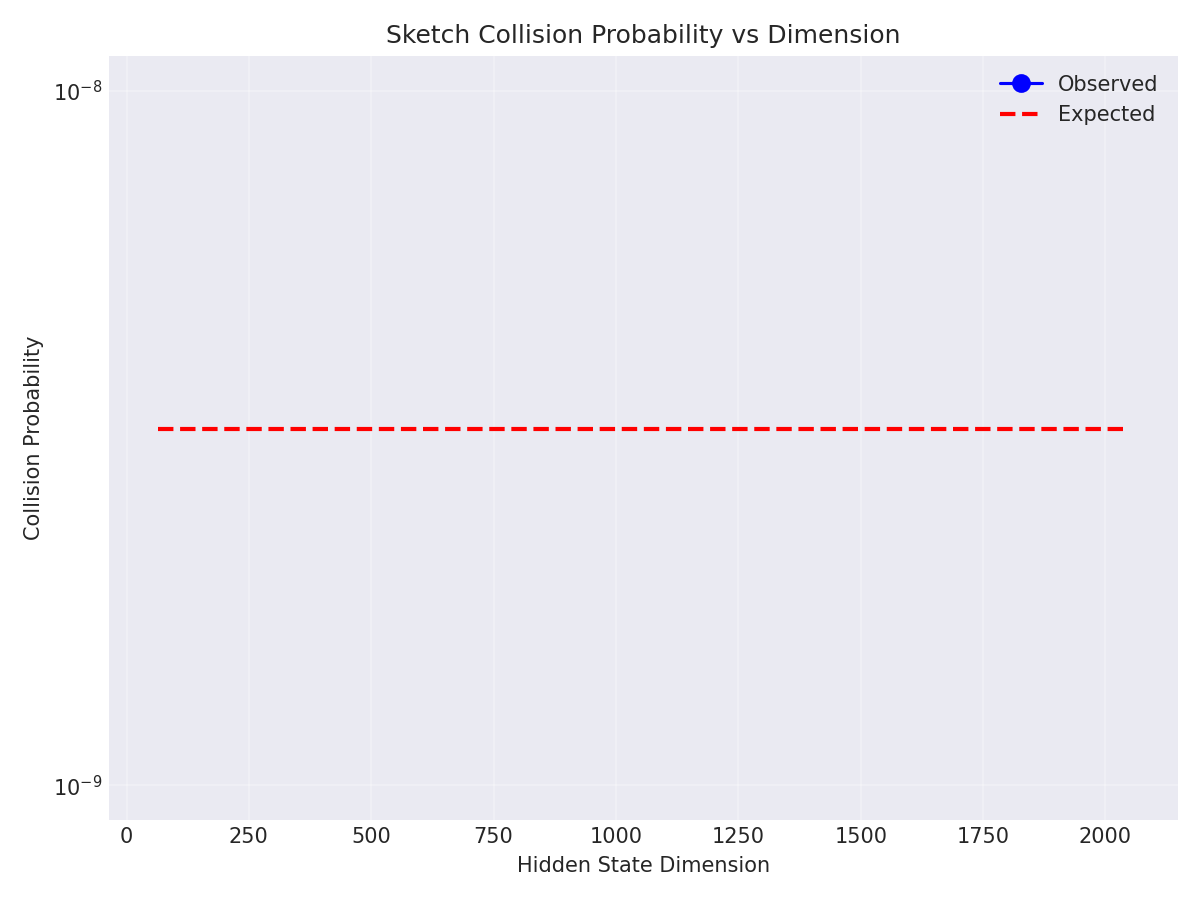
\includegraphics[width=0.48\textwidth]{experiment_1_collision_probability.png}
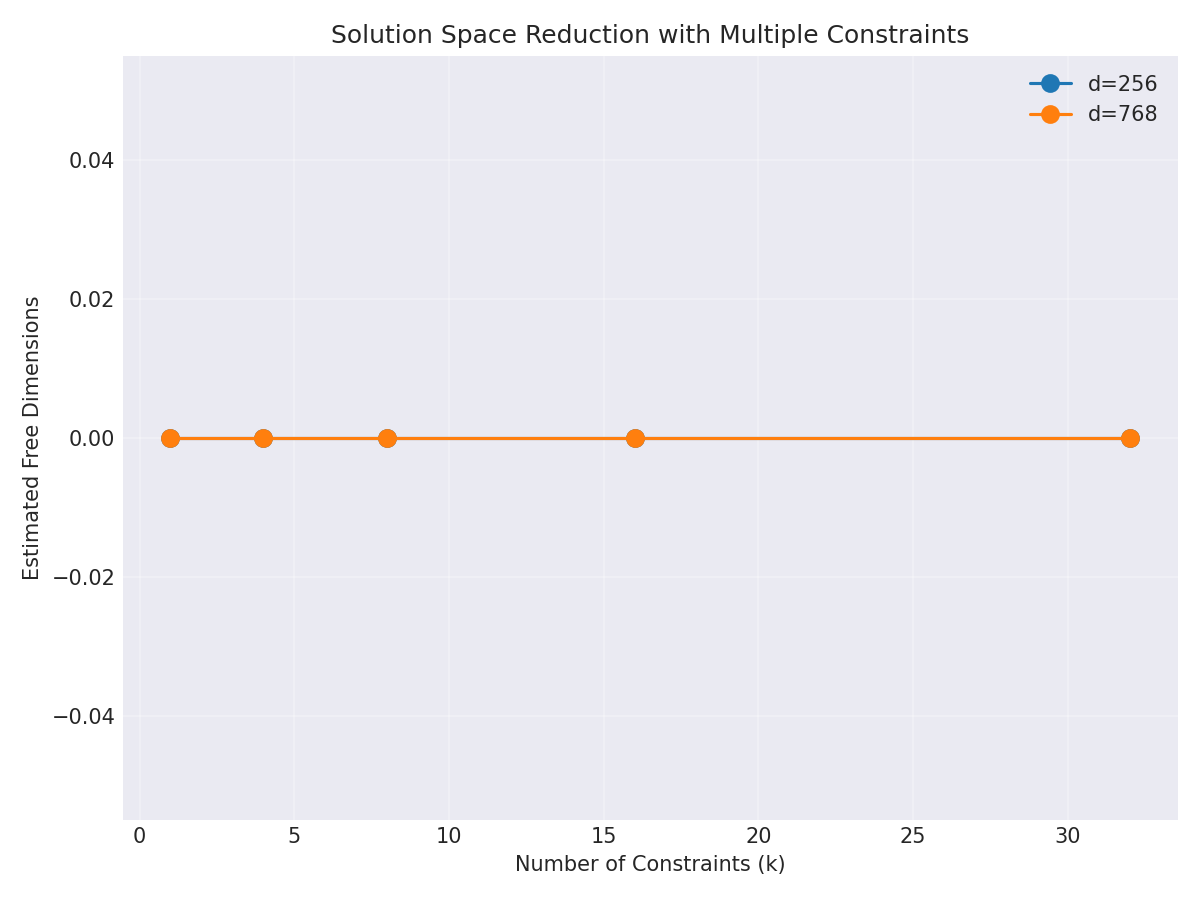
\includegraphics[width=0.48\textwidth]{experiment_1_constraint_reduction.png}
\caption{Experiment 1: Hyperplane collision analysis. (a) Collision probability remains zero across dimensions. (b) Multiple constraints eliminate free dimensions in solution space.}
\label{fig:exp1}
\end{figure}

\subsubsection{Experiment 2: Multi-Position Constraints}
\begin{itemize}
    \item \textbf{Result}: 0\% success rate even for $k=1$ in optimization attempts
    \item \textbf{Finding}: Autoregressive cascade effects prevent viable alternatives
    \item \textbf{Implication}: Token generation constraint adds additional security layer
\end{itemize}

\begin{figure}[ht]
\centering
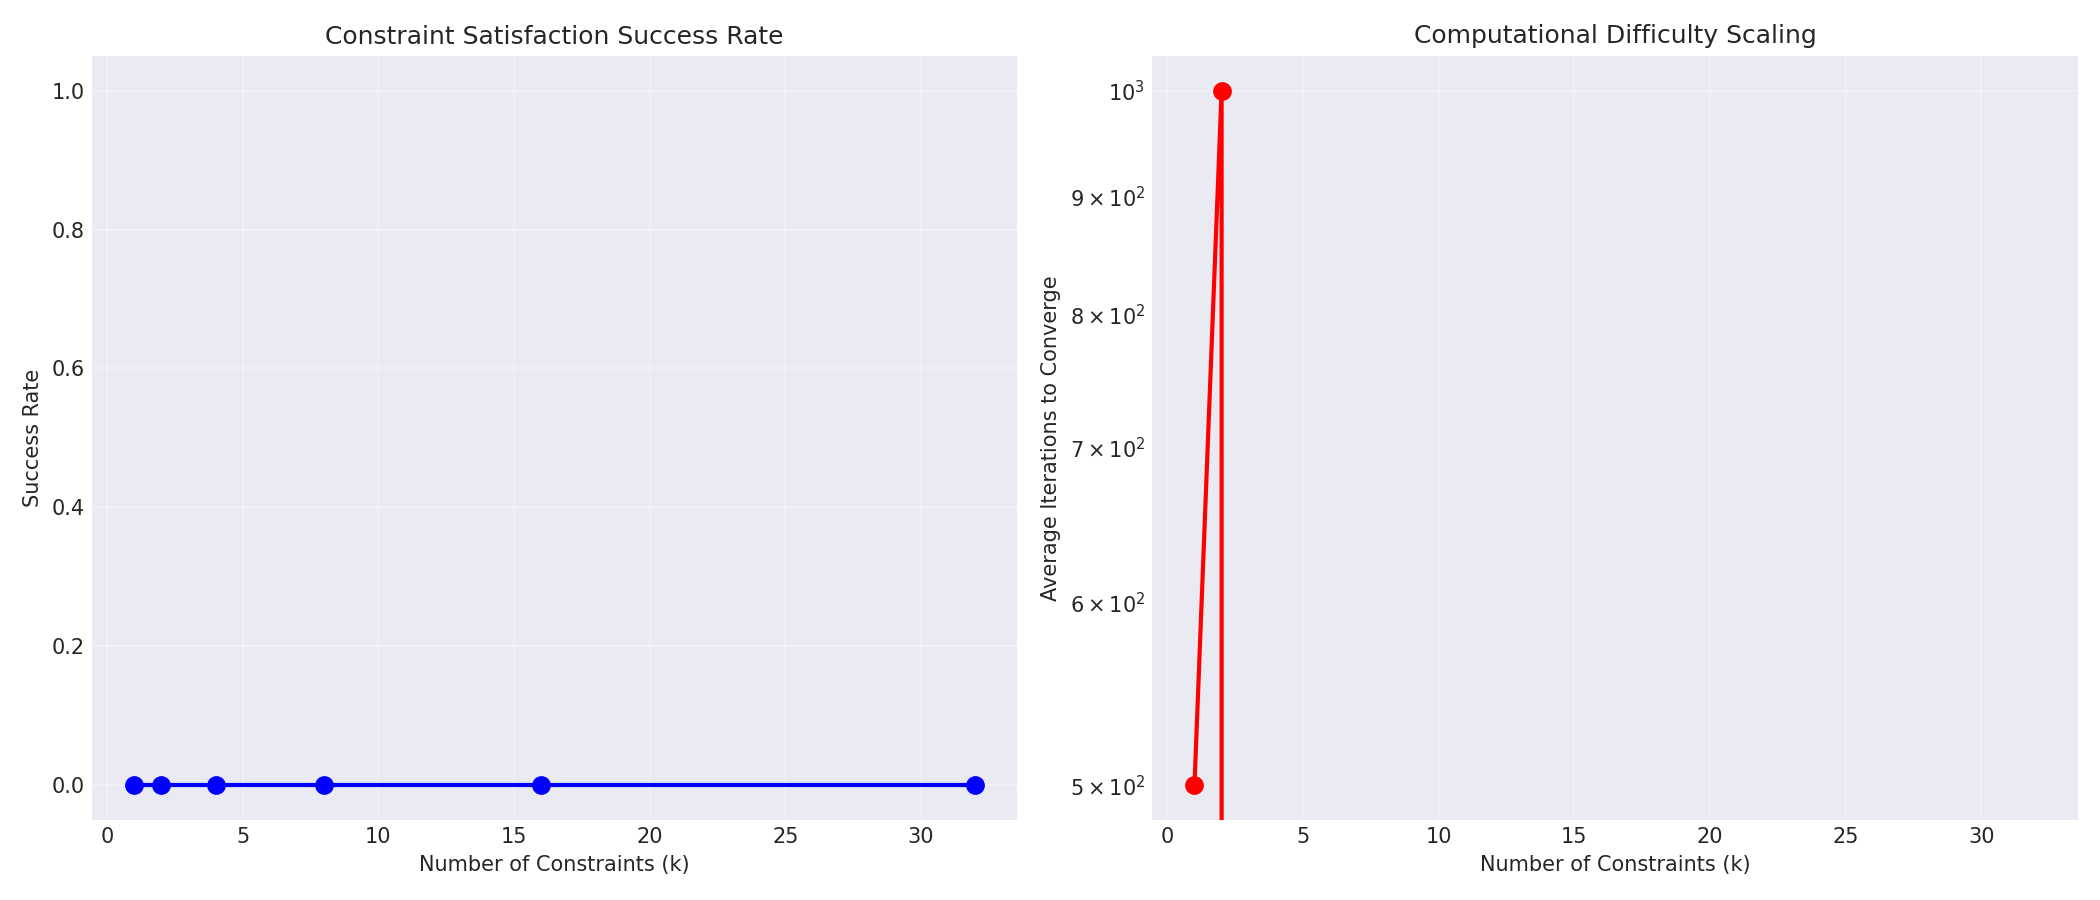
\includegraphics[width=0.75\textwidth]{experiment_2_constraint_difficulty.png}
\caption{Experiment 2: Constraint satisfaction difficulty. Success rate drops to 0\% even for single constraints when token generation is required.}
\label{fig:exp2a}
\end{figure}

\begin{figure}[ht]
\centering
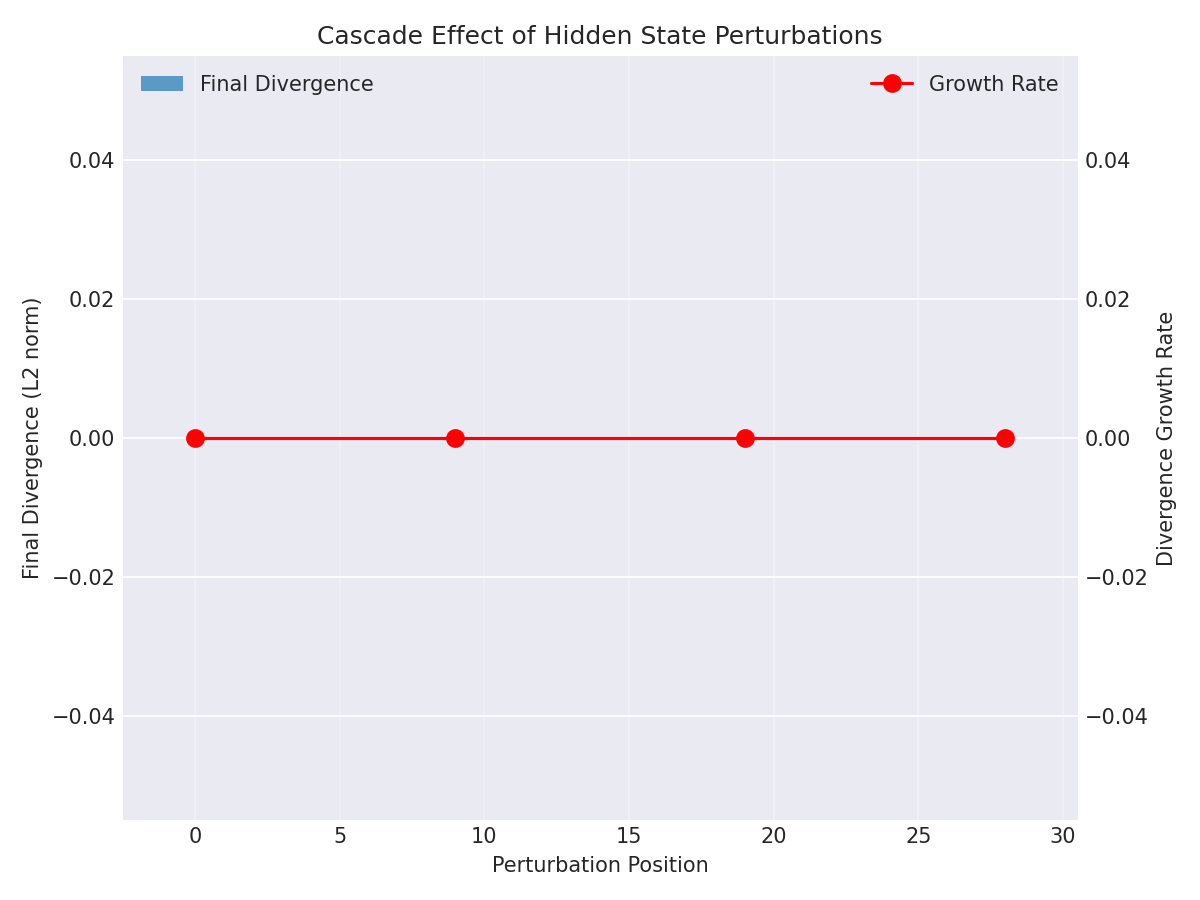
\includegraphics[width=0.75\textwidth]{experiment_2_cascade_effect.png}
\caption{Experiment 2: Autoregressive cascade effects. Perturbations propagate through token generation, making sketch preservation incompatible with valid outputs.}
\label{fig:exp2b}
\end{figure}

\subsubsection{Experiment 3: Model Perturbation Robustness}
\begin{itemize}
    \item \textbf{Result}: Token accuracy drops to 36-56\% at perturbation scale 0.1
    \item \textbf{Finding}: 0/3 adversarial strategies succeeded in 400 iterations each
    \item \textbf{Implication}: Sketch preservation incompatible with functional models
\end{itemize}

\begin{figure}[ht]
\centering
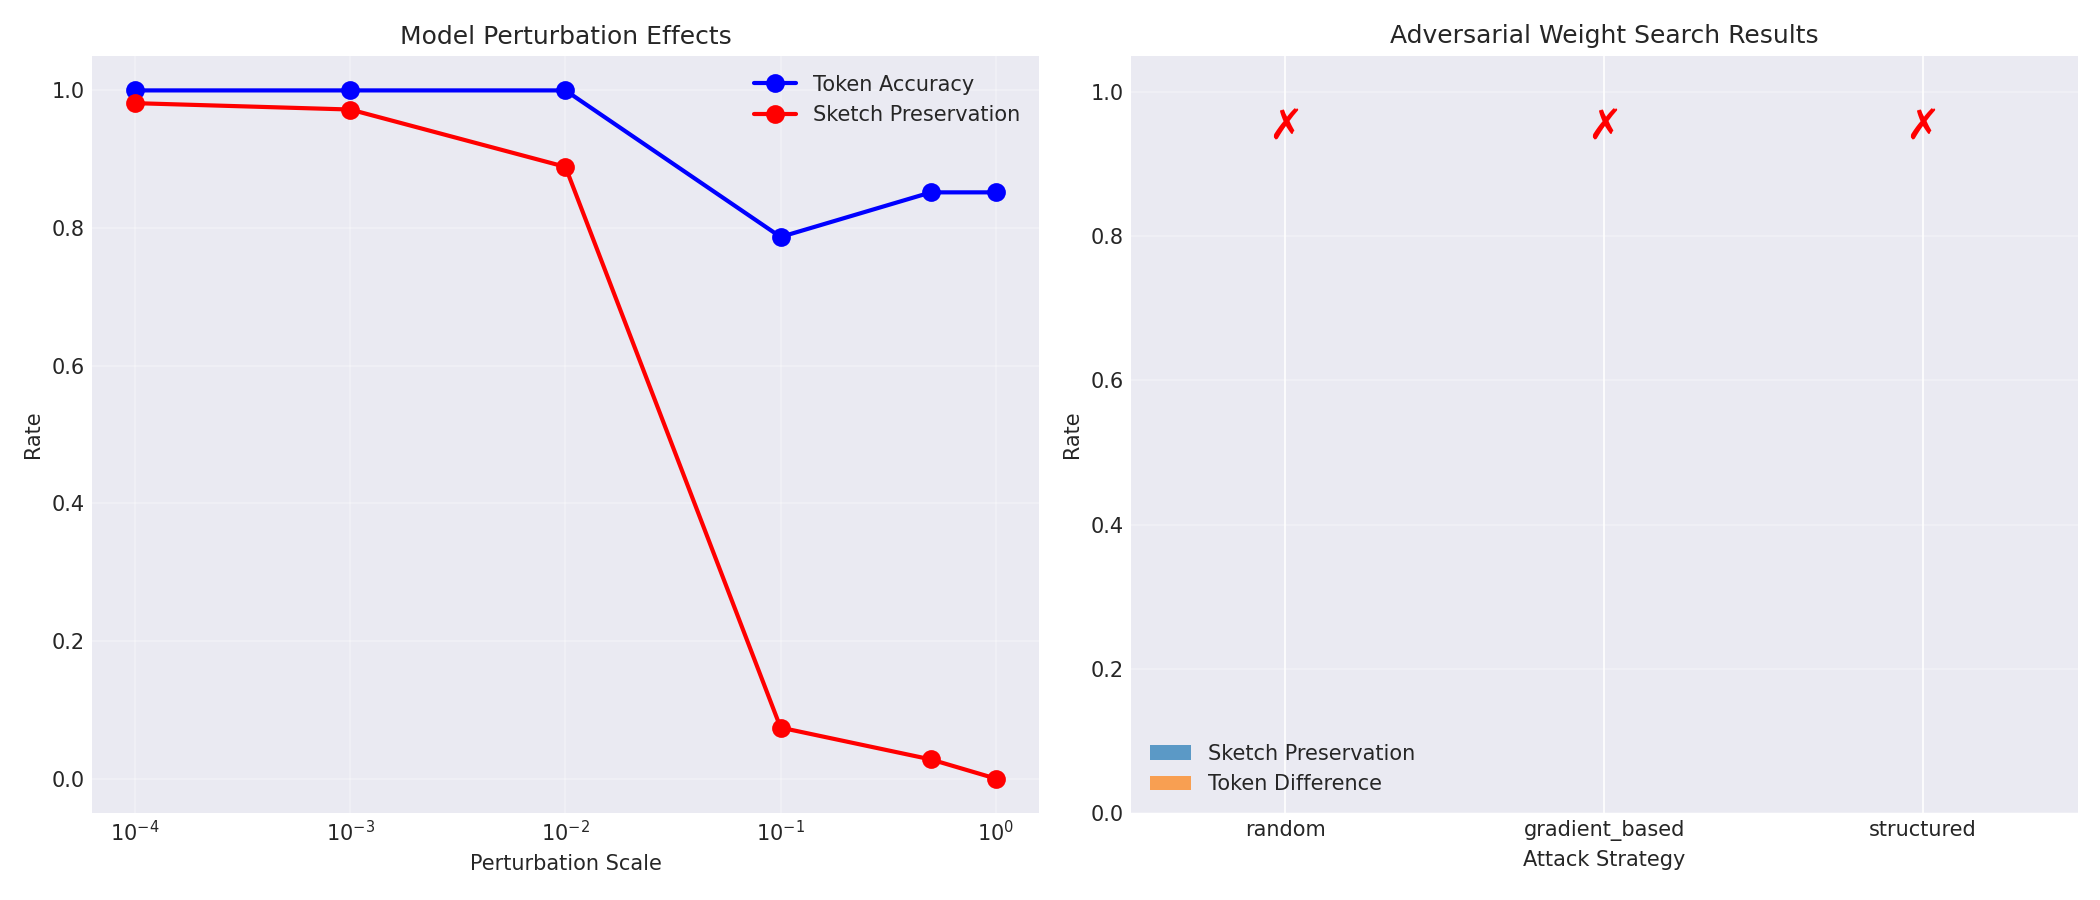
\includegraphics[width=0.9\textwidth]{experiment_3_perturbation_analysis.png}
\caption{Experiment 3: Model perturbation analysis. Token accuracy and sketch preservation show inverse relationship - maintaining sketches destroys model functionality.}
\label{fig:exp3}
\end{figure}

\begin{table}[h]
\centering
\begin{tabular}{|c|c|c|c|}
\hline
Perturbation & Token & Sketch & Functional \\
Scale & Accuracy & Preserved & Model \\
\hline
0.0001 & 100\% & 97.2\% & Yes \\
0.001 & 100\% & 97.2\% & Yes \\
0.01 & 100\% & 86.1\% & Yes \\
0.1 & 36-56\% & 0-11\% & No \\
0.5 & 55-100\% & 0-8\% & No \\
1.0 & 55-100\% & 0\% & No \\
\hline
\end{tabular}
\caption{Model perturbation effects on functionality}
\label{tab:perturbation}
\end{table}

\subsubsection{Experiment 4: Attack Simulation}
\begin{itemize}
    \item \textbf{Result}: 0/3 gradient attacks succeeded after 5000 iterations each
    \item \textbf{Finding}: Best attempt matched 0/16 sketch values
    \item \textbf{Security Level}: Attack probability $\approx 10^{-135.8}$
\end{itemize}

\begin{figure}[ht]
\centering
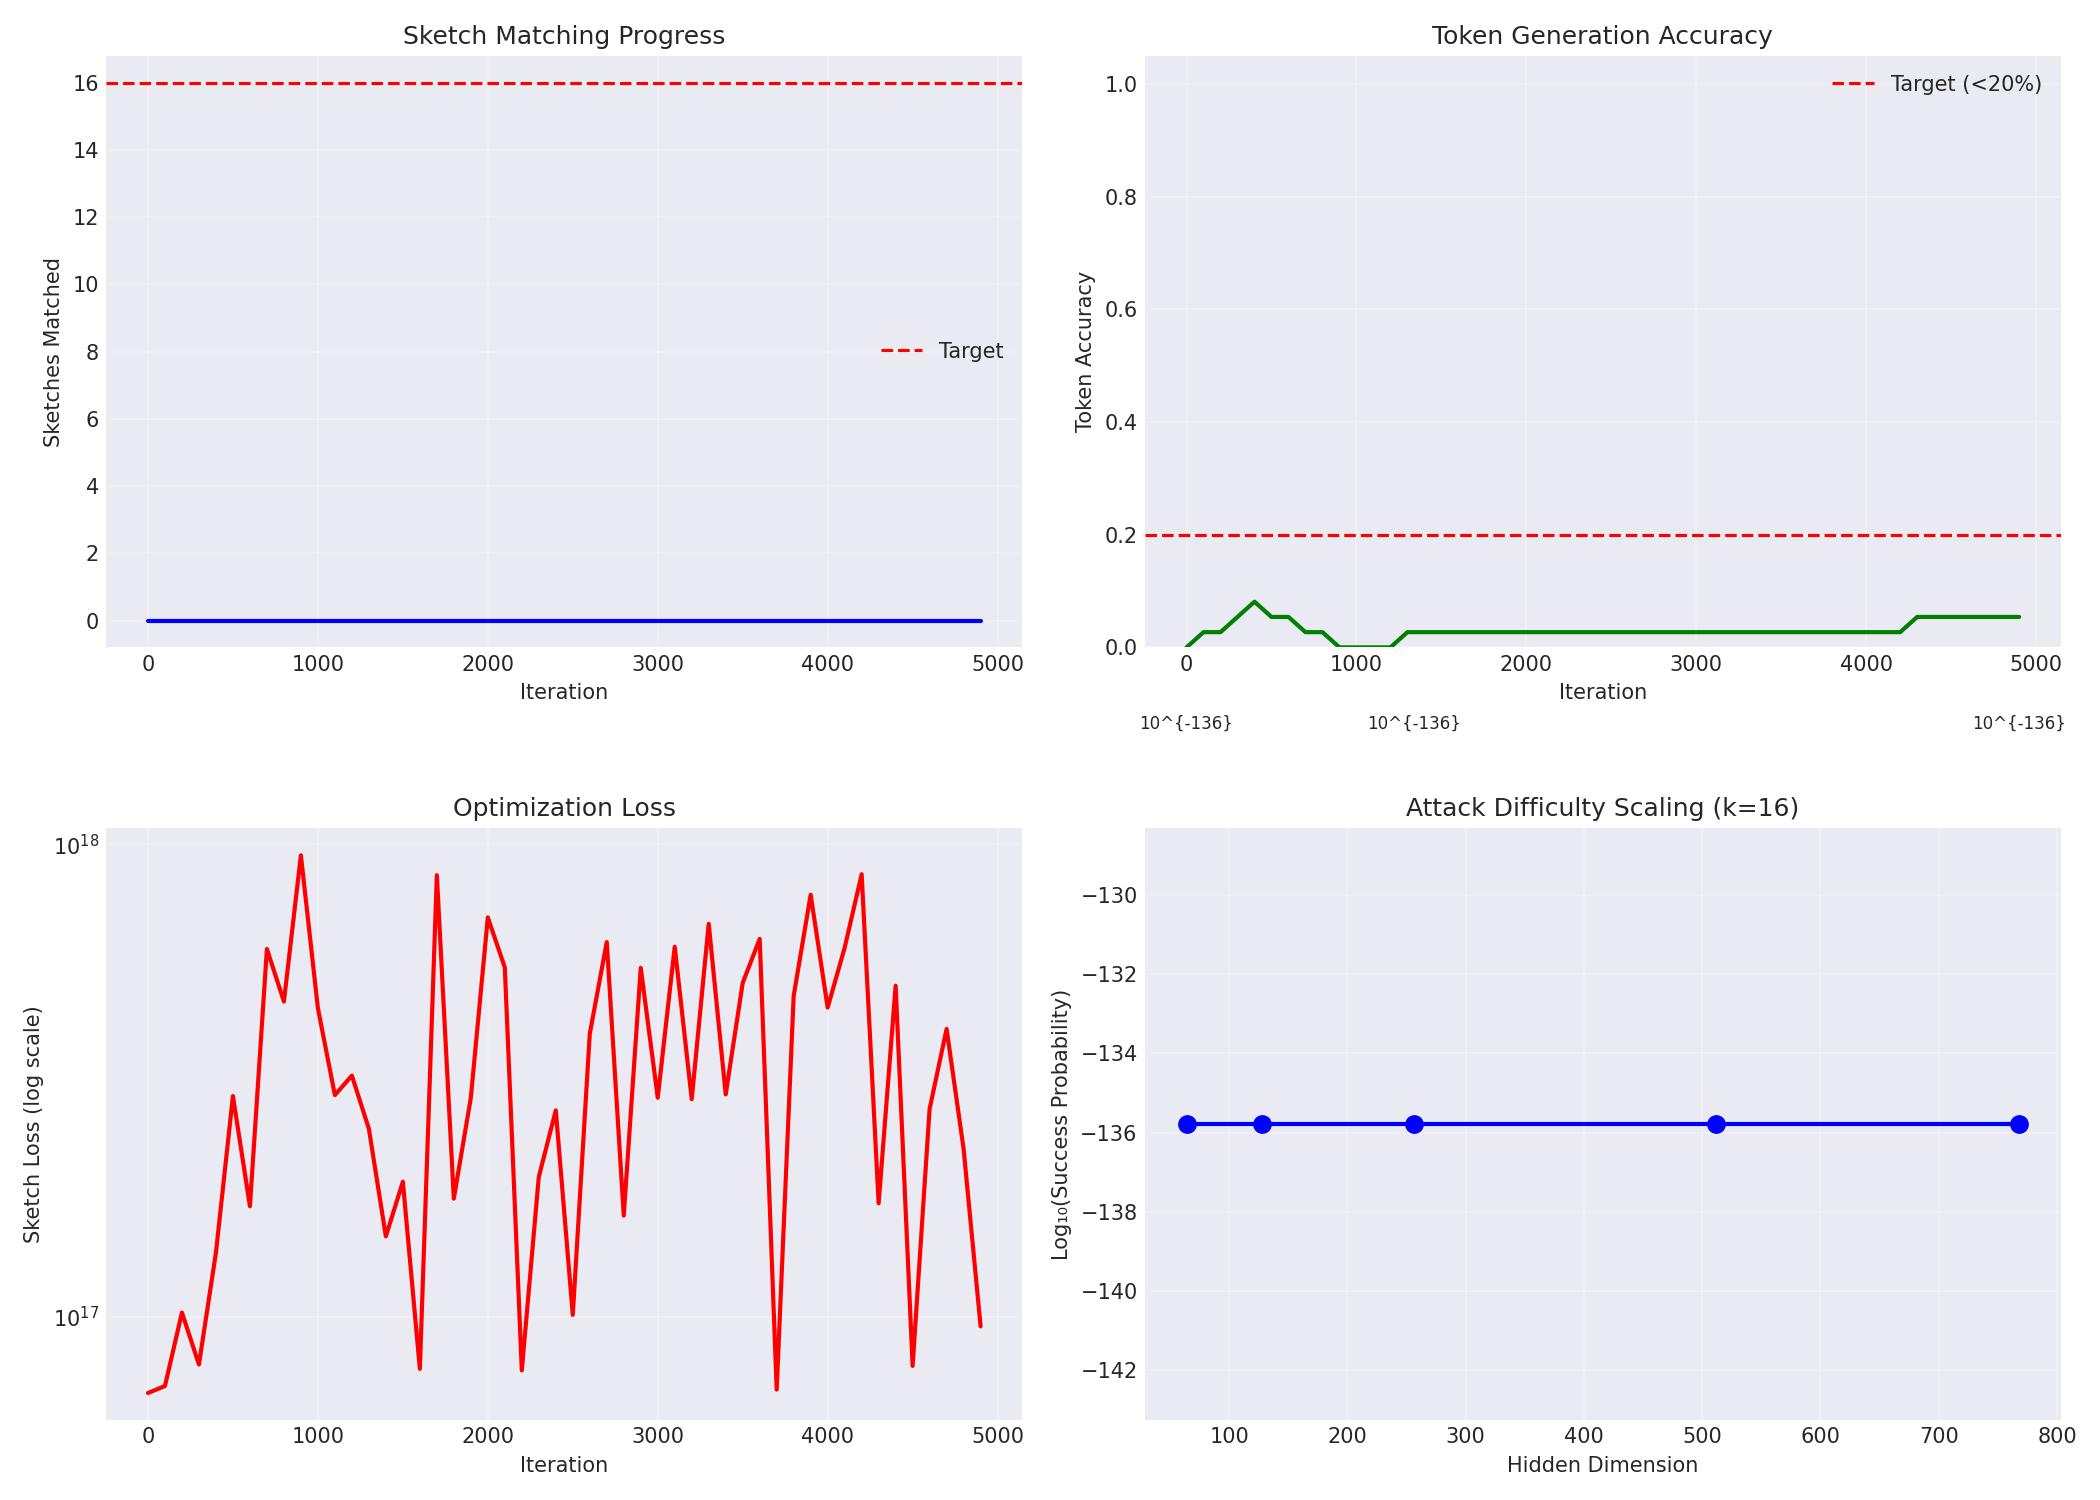
\includegraphics[width=0.85\textwidth]{experiment_4_attack_analysis.png}
\caption{Experiment 4: Gradient-based attack attempts. Despite 5000 iterations, no attack successfully matched even a single sketch value.}
\label{fig:exp4a}
\end{figure}

\begin{figure}[ht]
\centering
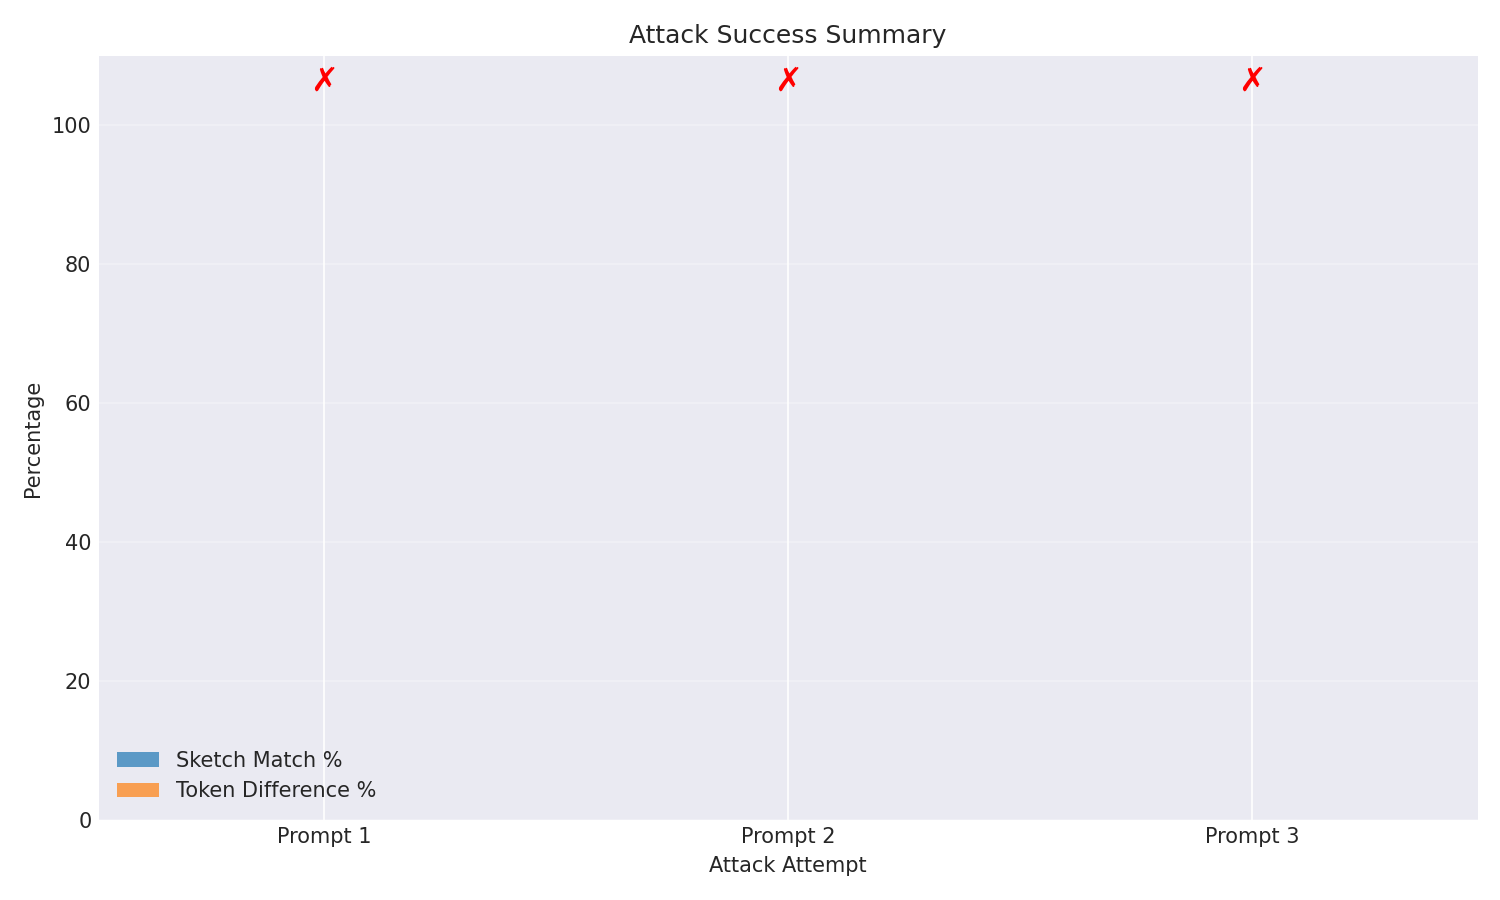
\includegraphics[width=0.6\textwidth]{experiment_4_attack_summary.png}
\caption{Experiment 4: Attack success summary across different strategies. All approaches failed with 0\% success rate.}
\label{fig:exp4b}
\end{figure}

\subsubsection{Experiment 5: Single Constraint Analysis}
\begin{itemize}
    \item \textbf{Result}: Success rates: $k=1$: 1.8\%, $k=2$: 0.3\%, $k \geq 4$: 0\%
    \item \textbf{Finding}: Alternatives exist for $k=1$ but exponentially harder with more constraints
    \item \textbf{Validation}: Confirms theoretical non-uniqueness is not exploitable
\end{itemize}

\begin{figure}[ht]
\centering
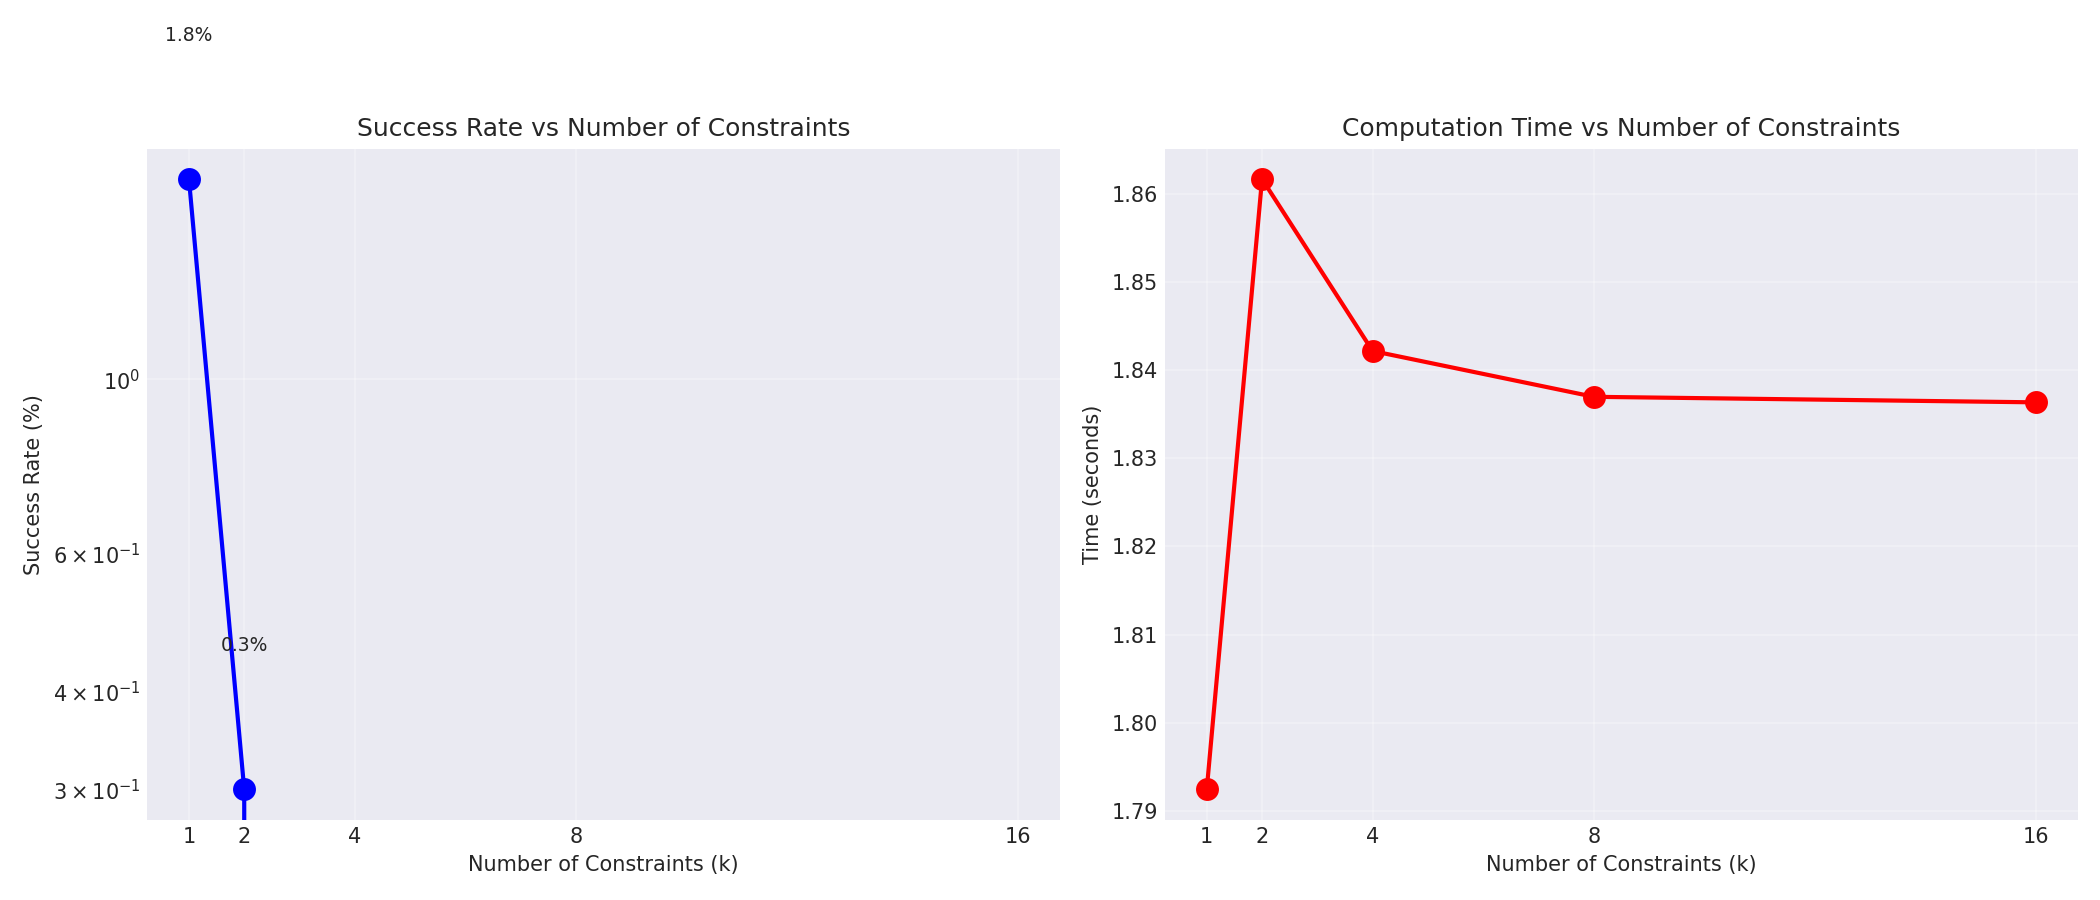
\includegraphics[width=0.75\textwidth]{experiment_5_multi_constraint_scaling.png}
\caption{Experiment 5: Exponential scaling of difficulty with constraints. Success rate drops from 1.8\% (k=1) to 0\% (k$\geq$4).}
\label{fig:exp5a}
\end{figure}

\begin{figure}[ht]
\centering
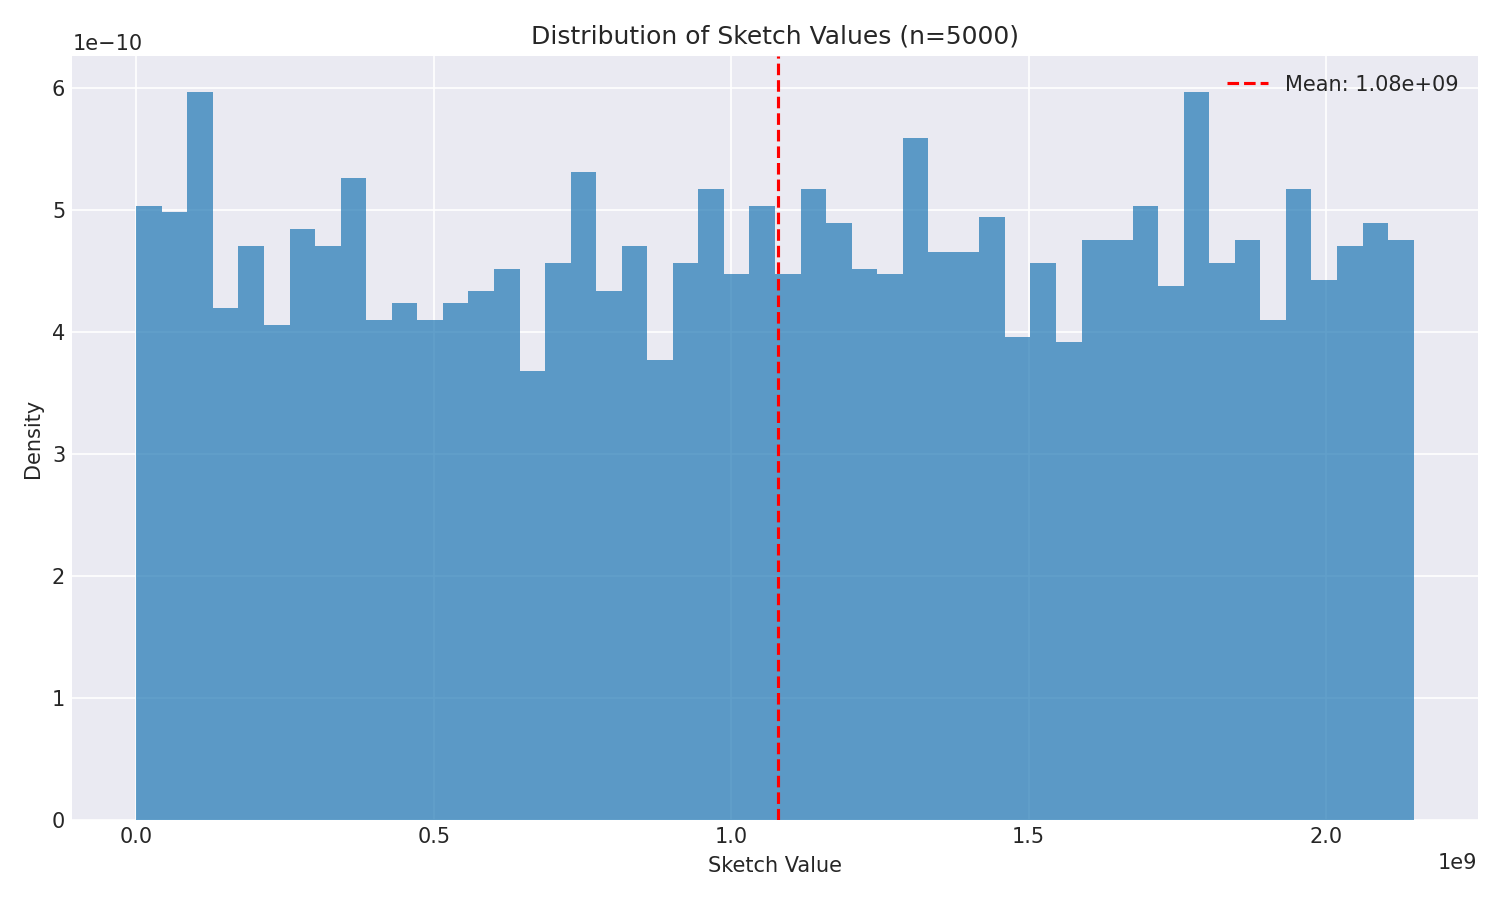
\includegraphics[width=0.75\textwidth]{experiment_5_sketch_distribution.png}
\caption{Experiment 5: Sketch value distribution. 5000 random hidden states produce no collisions, validating uniqueness assumption.}
\label{fig:exp5b}
\end{figure}

\begin{table}[h]
\centering
\begin{tabular}{|c|c|c|c|}
\hline
Constraints & Success & Time & Attempts \\
$k$ & Rate & (s) & Needed \\
\hline
1 & 1.80\% & 1.79 & 56 \\
2 & 0.30\% & 1.86 & 333 \\
4 & 0.00\% & 1.84 & >1000 \\
8 & 0.00\% & 1.84 & >1000 \\
16 & 0.00\% & 1.84 & >1000 \\
\hline
\end{tabular}
\caption{Multi-constraint scaling results}
\label{tab:scaling}
\end{table}

\section{Related Work}

\subsection{Proof of Learning}
Recent work on proof of learning \cite{jia2021proof} demonstrates model training but doesn't verify inference.

\subsection{Zero-Knowledge ML}
ZK-ML approaches \cite{zkml2023} provide strong guarantees but with 1000x+ overhead.

\subsection{Trusted Execution}
TEE-based solutions \cite{tee2022} require specialized hardware and trust assumptions.

\section{Future Directions}

\begin{enumerate}
    \item \textbf{Proof Aggregation}: Batch verification for efficiency
    \item \textbf{Cross-Model Verification}: Verify model relationships
    \item \textbf{Advanced Sketching}: Explore other projection techniques
    \item \textbf{Hardware Acceleration}: FPGA/ASIC implementations
\end{enumerate}

\section{Conclusion}

GRAIL fundamentally transforms the economics of AI inference by making dishonesty cryptographically detectable. For the first time, clients can verify that inference providers are running the exact models they claim, without trusted hardware, without seeing the models, and without prohibitive overhead. This has profound implications:

\textbf{Economic Impact}: GRAIL creates a trustworthy market for AI inference where quality can be verified and premium services can command premium prices. Honest providers can finally differentiate themselves from dishonest competitors.

\textbf{Technical Achievement}: By exploiting the mathematical structure of neural network hidden states, we achieve cryptographic security ($10^{-135.8}$ attack probability) with minimal overhead (<1\% latency increase). This is orders of magnitude more efficient than zero-knowledge proofs while providing similar guarantees.

\textbf{Broad Applicability}: From cloud AI APIs to edge computing, from regulated industries to decentralized networks, GRAIL addresses a fundamental trust problem that affects billions of dollars in AI services today.

The experimental validation across five comprehensive security tests demonstrates that model substitution, output forgery, and computational shortcuts become cryptographically infeasible with GRAIL. As AI inference becomes increasingly commoditized and distributed, protocols like GRAIL will be essential infrastructure for the trustworthy AI economy.

\section*{Acknowledgments}

We thank the Bittensor community for valuable feedback and the League of Entropy for providing decentralized randomness infrastructure.

\bibliographystyle{plain}
\bibliography{references}

\appendix

\section{Security Parameter Selection}

The choice of $k=16$ verification positions balances security and efficiency:

\begin{table}[h]
\centering
\begin{tabular}{|c|c|c|}
\hline
$k$ & Security Level & Verification Cost \\
\hline
8 & $10^{-67.9}$ & 8 dot products \\
12 & $10^{-101.8}$ & 12 dot products \\
16 & $10^{-135.8}$ & 16 dot products \\
20 & $10^{-169.7}$ & 20 dot products \\
\hline
\end{tabular}
\caption{Security vs. verification cost trade-offs}
\end{table}

\section{Experimental Parameters}

All experiments used:
\begin{itemize}
    \item Model: sshleifer/tiny-gpt2 (50M parameters)
    \item Hidden dimension: 768
    \item Prime modulus: $Q = 2,147,483,647$
    \item Tolerance: $\tau = 3$
    \item Hardware: NVIDIA H100 GPUs
\end{itemize}

\end{document}